\chapter{Physics of lepton colliders}
\label{Lepton_Physics}
\begin{chapterabstract}
The physics done at particle colliders, where two particle beams are brought into collision, is the physics of atoms and quanta, of nuclei and partons, of particles that build up everything we know, but also of new particles, physics beyond our current knowledge.
After a brief introduction of the Standard Model, a theory describing the elementary particles and the fundamental forces, the physics processes at a lepton collider will be explained in more detail.
\end{chapterabstract}
\newline

Particle physics reaches back to the ancient Greek times, when the idea was developed that matter is made of ``indivisible'' (\'atomos, Greek) parts.
Atoms are, in fact, not indivisible at all.
When the electron was experimentally discovered in 1897 by J.J. Thomson, it was proposed that these particles are part of atoms.
\section{The Standard Model}
\label{StandardModel}
\section{Production modes}
\label{Production_modes}
\section{Backgrounds}
\label{Backgrounds}
\subsection{High cross-section backgrounds from beam-beam interactions}
\label{BeamBeam}
\subsubsection{Pair background}
\label{BeamBeam:pairs}

\begin{figure}
\begin{subfigure}[b]{0.33\textwidth}
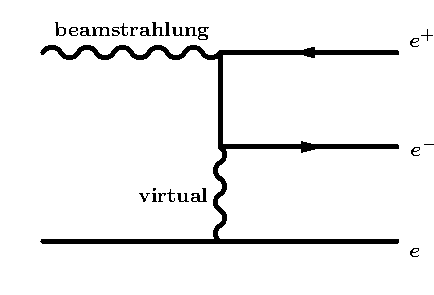
\includegraphics[width=\textwidth]{Figures/Bethe-Heitler.pdf}
\caption{Bethe-Heitler}
\end{subfigure}
\begin{subfigure}[b]{0.33\textwidth}
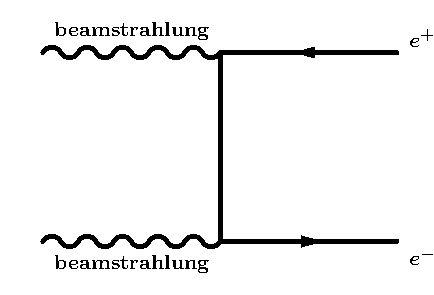
\includegraphics[width=\textwidth]{Figures/Breit-Wheeler.pdf}
\caption{Breit-Wheeler}
\end{subfigure}
\begin{subfigure}[b]{0.33\textwidth}
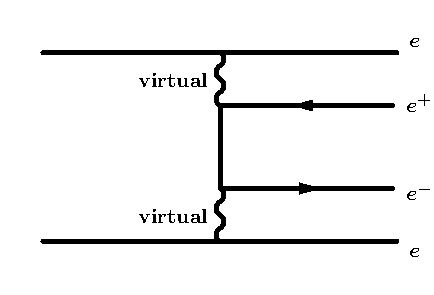
\includegraphics[width=\textwidth]{Figures/Landau-Lifshitz.pdf}
\caption{Landau-Lifschitz}
\end{subfigure}
\caption[LO Feynman diagrams of the production of the background pairs.]{The LO Feynman diagrams of the production processes of the background pairs: Bethe-Heitler, Breit-Wheeler and Landau-Lifschitz.}
\label{fig:Feynman:pair_production}
\end{figure}

\subsubsection{Bhabha scattering and $\gamma\gamma\rightarrow$hadrons}
\label{BeamBeam:bhabha_gammagamma}

\begin{figure}
\centering
\begin{subfigure}[b]{0.35\textwidth}
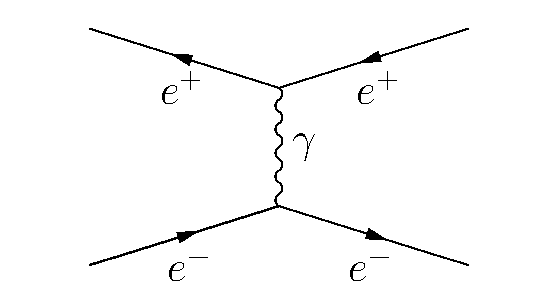
\includegraphics[width=\textwidth]{Figures/bhabha_scattering.pdf}
\caption{Bhabha scattering}
\end{subfigure}
\vspace*{0.2cm}
\begin{subfigure}[b]{0.35\textwidth}
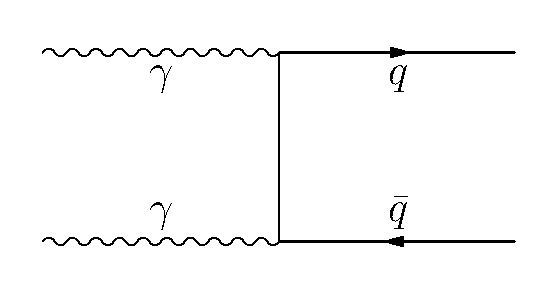
\includegraphics[width=\textwidth]{Figures/gammagamma_hadrons.pdf}
\caption{$\gamma\gamma\rightarrow$hadrons}
\end{subfigure}
\caption[LO Feynman diagrams of bhabha scattering and the $\gamma\gamma\rightarrow$hadrons process.]{The LO Feynman diagrams of the bhabha scattering and the $\gamma\gamma\rightarrow$hadrons process.}
\label{fig:Feynman:bhabha_gammagamma}
\end{figure}

\subsection{Machine backgrounds}
\label{MachineBackgrounds}